%\graphicspath{{./Plots/}}


\documentclass[conference]{IEEEtran}
%%%%%%%%%%%%%%%%%%%%%%%%%%%%%%%%%%%%%%%%%%%%%%%%%%%%%%%%%%%%%%%%%%%%%%%%%%%%%%%%%%%%%%%%%%%%%%%%%%%%%%%%%%%%%%%%%%%%%%%%%%%%%%%%%%%%%%%%%%%%%%%%%%%%%%%%%%%%%%%%%%%%%%%%%%%%%%%%%%%%%%%%%%%%%%%%%%%%%%%%%%%%%%%%%%%%%%%%%%%%%%%%%%%%%%%%%%%%%%%%%%%%%%%%%%%%
\usepackage{amssymb}
\usepackage{amsmath}
\usepackage{geometry}
\usepackage{graphicx}
\usepackage{amsfonts}

\setcounter{MaxMatrixCols}{10}
%TCIDATA{OutputFilter=LATEX.DLL}
%TCIDATA{Version=5.50.0.2960}
%TCIDATA{<META NAME="SaveForMode" CONTENT="1">}
%TCIDATA{BibliographyScheme=BibTeX}
%TCIDATA{Created=Wednesday, December 09, 2020 21:10:24}
%TCIDATA{LastRevised=Tuesday, December 15, 2020 21:43:29}
%TCIDATA{<META NAME="GraphicsSave" CONTENT="0">}
%TCIDATA{<META NAME="DocumentShell" CONTENT="Articles\SW\IEEE Transactions for Conferences">}
%TCIDATA{Language=American English}
%TCIDATA{CSTFile=IEEEtran.cst}

\graphicspath{{c:/Users/lin11/OneDrive/Documents/JHU-DESKTOP-MR0GT8B/adversarial_examples/}}
\newtheorem{theorem}{Theorem}
\newtheorem{acknowledgement}[theorem]{Acknowledgement}
\newtheorem{algorithm}[theorem]{Algorithm}
\newtheorem{axiom}[theorem]{Axiom}
\newtheorem{case}[theorem]{Case}
\newtheorem{claim}[theorem]{Claim}
\newtheorem{conclusion}[theorem]{Conclusion}
\newtheorem{condition}[theorem]{Condition}
\newtheorem{conjecture}[theorem]{Conjecture}
\newtheorem{corollary}[theorem]{Corollary}
\newtheorem{criterion}[theorem]{Criterion}
\newtheorem{definition}[theorem]{Definition}
\newtheorem{example}[theorem]{Example}
\newtheorem{exercise}[theorem]{Exercise}
\newtheorem{lemma}[theorem]{Lemma}
\newtheorem{notation}[theorem]{Notation}
\newtheorem{problem}[theorem]{Problem}
\newtheorem{proposition}[theorem]{Proposition}
\newtheorem{remark}[theorem]{Remark}
\newtheorem{solution}[theorem]{Solution}
\newtheorem{summary}[theorem]{Summary}
\input{tcilatex}
\begin{document}

\title{Generating and defending against adversarial examples in
vision-optimized neural architectures}
\pubid{\copyright ~2020 }
\specialpapernotice{}
\date{December 9, 2020}

%TCIMACRO{%
%\TeXButton{Author Information}{\author{\authorblockN{Daniel Donoghue}
%\authorblockA{
%Email: ddonogh1@jhu.edu}
%\and
%\authorblockN{Nicholas Lines}
%\authorblockA{
%Email: nicholasalines@gmail.com}
%\and
%\authorblockN{Arnaldo Pereira}
%\authorblockA{
%Email: aepereira@gmail.com}
%}}}%
%BeginExpansion
\author{\authorblockN{Daniel Donoghue}
\authorblockA{
Email: ddonogh1@jhu.edu}
\and
\authorblockN{Nicholas Lines}
\authorblockA{
Email: nicholasalines@gmail.com}
\and
\authorblockN{Arnaldo Pereira}
\authorblockA{
Email: aepereira@gmail.com}
}%
%EndExpansion

%TCIMACRO{\TeXButton{Make Title}{\maketitle}}%
%BeginExpansion
\maketitle%
%EndExpansion

%TCIMACRO{\TeXButton{Begin abstract}{\begin{abstract}}}%
%BeginExpansion
\begin{abstract}%
%EndExpansion

As automated decision-making becomes more popular and more dependent upon
artificial intelligence, securing sensitive models from adversarial behavior
has become essential. Neural networks are particularly vulnerable to
so-called adversarial examples \cite{szegedy2014intriguing}, and various
attacks and defenses have been explored in the literature.

Our intention in this paper is to demonstrate and confirm the results of
such attacks at an informative but modest scale. We apply two common attacks
to both the Wide ResNet and GoogLeNet neural models, and test two defenses,
in a reproducible computational environment. We show that significant
improvements in network robustness are available with minimal defense
measures.

The authors are listed alphabetically, and all made equal contributions.
This work is performed in association with the Johns Hopkins Engineering for
Professionals Program, as a project for EN.625.638.8VL2.FA20 Neural Networks.

All code and further reference materials are available online at
https://github.com/linesn/adversarial\_examples. This repository serves as
an extensive appendix to the report given here.

%TCIMACRO{\TeXButton{End abstract}{\end{abstract}}}%
%BeginExpansion
\end{abstract}%
%EndExpansion

%TCIMACRO{\TeXButton{Table of Contents}{\tableofcontents}}%
%BeginExpansion
\tableofcontents%
%EndExpansion

\bigskip

\section{Executive Summary}

Since 2014 when Szegedy et al \cite{szegedy2014intriguing} published the
first observation on the subject, adversarial examples have gained much
attention in both the study of adversarial machine learning research and the
more results-oriented world of practical neural architecture, due to the
alarming weaknesses they expose and the interesting robustness that can be
introduced via defense efforts. The term \textquotedblleft adversarial
example\textquotedblright\ is used to describe \textquotedblleft an input to
a machine learning model that is intentionally designed to cause the model
to make a mistake in its predictions, despite resembling a valid input to a
human\textquotedblright\ \cite{wiyatno2019adversarial}. As such these
examples are classed as evasion techniques by adversarial machine learning
theory, since their goal is to evade detection while producing
misinterpretations \cite{wiki:aml}.

Most of the literature on the subject (in keeping with traditions in the
neural network community) uses image recognition tasks to demonstrate the
efficacy of attacks and defenses, and we will do the same. In this paper we
will demonstrate successful us of the Fast Gradient Sign Method (FGSM) \cite%
{goodfellow2014explaining} and Directed Gradient Sign (DGSM) \cite%
{madry2020adversarial} attacks against convolutional neural networks trained
with Imagenette data. We will then examine the results of applying two
common defenses: first, perturbed prediction averaging, and second, training
using adversarial examples. We confirm the observations of Goodfellow et al 
\cite{goodfellow2014explaining} and show that, while the Wide ResNet and
GoogLeNet architectures are very susceptible to the above attacks, the named
defenses also produce significant improvement to the robustness of the
classifiers.

\section{Project overview}

\subsection{Why are adversarial examples effective?}

In practice neural architectures based on linear components are preferred
(over, for example, radial basis components) because of their speed in
training and inference. However, it is this property that makes them
particularly vulnerable to the most common form of adversarial example \cite%
{goodfellow2014explaining}. Neural classifier inputs or features naturally
have some precision limit, such as a color range or pixel count, below which
perturbations are ignored. Consider an input vector $\mathbf{X}$, to which
we add a noise vector $\mathbf{\eta }$, where every $\eta \in \mathbf{\eta }$
is smaller than $\epsilon ,$ the precision limit. To humans and a first pass
review by machines, $\mathbf{X}$ and $\mathbf{X+\eta }$ are identical.
However, when the linear activity function is computed, the network's
weights are dotted with the input, yielding approximately 
\begin{equation*}
\mathbf{W}^{\intercal }(\mathbf{X+\eta )=W}^{\intercal }\mathbf{X+W}%
^{\intercal }\mathbf{\eta ,}
\end{equation*}%
where the noise term $\mathbf{W}^{\intercal }\mathbf{\eta }$ can grow very
large if $\mathbf{W}$ is ill-conditioned. This means, in practice, that
networks reliant on linear activity functions can produce extremely
different outputs when given only minimally altered inputs, as shown in
Figure \ref{example}. 
\begin{figure*}[h]
\centering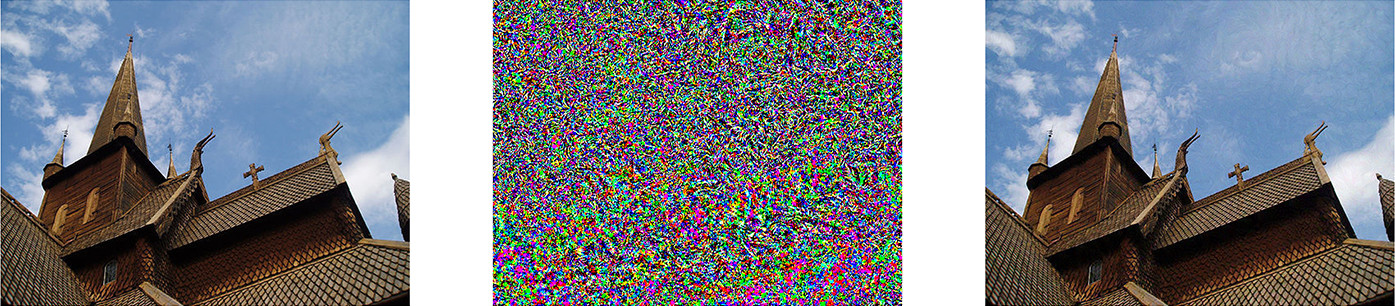
\includegraphics{{Plots/plots_base/adversarial_example_nocap.jpg}}
\caption{An adversarial example. The original Imagenette photograph on the
left is altered by adding the noise shown in the center (which is scaled up
to make it visible). The resulting image on the right appears identical to
the original, but is misidentified by the classifier.}
\label{example}
\end{figure*}
An adversarial example. The original Imagenette photograph on the left is
altered by adding the noise shown in the center (which is scaled up to make
it visible). The resulting image on the right appears identical to the
original, but is misidentified by the classifier.

\subsection{Attacks}

The FGSM attack \cite{goodfellow2014explaining} takes advantage of this
weakness in a straightforward manner. The attacker forms the perturbation
vector $\mathbf{\eta }$ to match the cost function gradient sign for a given
input, computing 
\begin{equation*}
\mathbf{\eta }=\epsilon _{\ast }\text{sign}(\nabla _{\mathbf{X}}J(\mathbf{%
\theta },\mathbf{X},y))
\end{equation*}%
where $\epsilon _{\ast }$ is the allowable level of perturbation, $J$ is the
network cost function, $\mathbf{\theta }$ is the vector of model parameters,
and $y$ is the true label. Thus, if the attacker is in possession of the
model and labeled training data, it is easy to train the network to behave
badly using simple backpropagation. The result is that the network will lose
certainty in the true label classification, and often misclassify the data
at random. The attack parameter $\epsilon _{\ast }$ may be scaled, of
course, but making $\epsilon _{\ast }$ much larger than the network
precision level $\epsilon $ may produce examples whose alteration is visible
to human reviewers, so smaller $\epsilon _{\ast }$ are desirable from the
adversarial perspective.

One can alter this attack to cause the network to favor a particular class
instead \cite{madry2020adversarial}. We will call this the Directed Gradient
Sign Method (DGSM). This time we use the loss function to direct the network
toward a specific desired label. We iterate using gradient descent for a
given number of iterations, and project the gradient onto the $l_{\infty }$%
-norm $\epsilon _{\ast }$-sphere, which has the effect of insisting that a
feature is not altered by more than $\epsilon _{\ast }$. For a given input $%
\mathbf{X}$, the attacker must solve the minimization problem 
\begin{eqnarray*}
\min_{\delta }\{J_{adv}(\mathbf{X}+\mathbf{\delta }) &=&J(\mathbf{\theta },%
\mathbf{X}+\mathbf{\delta },y_{desired}) \\
&&-J(\mathbf{\theta },\mathbf{X}+\mathbf{\delta },y_{true})\}\text{ } \\
\text{subject to }\left\vert \left\vert \mathbf{\delta }\right\vert
\right\vert _{\infty } &\leq &\epsilon _{\ast }
\end{eqnarray*}%
where $J$ is again the loss function, $\mathbf{\theta }$ the fixed network
parameters, $y_{desired}$ and $y_{true}$ are two different labels, and $%
\mathbf{\delta }$ is the directed perturbation vector. This requires using
forward passes and backpropagation within the network over $N$ iterations,
applying the update rule%
\begin{eqnarray*}
\mathbf{\delta }_{t} &=&\mathbf{\delta }_{t-1}-a\text{ sign}(\nabla L_{adv}(%
\mathbf{X}+\mathbf{\delta }_{t-1})), \\
\mathbf{\delta }_{t} &\leftarrow &\text{clip}(\mathbf{\delta }_{t},-\epsilon
_{\ast },\epsilon _{\ast })
\end{eqnarray*}%
beginning with the zero vector $\mathbf{\delta }_{0}=\mathbf{0}$. The result
of this attack is that the classifier will incorrectly favor the chosen
label $y_{desired}$ in adversarial inputs, despite remaining perfectly
capable of correctly classifying unaltered inputs.

\subsection{Defenses}

A theme that has emerged in the literature is that there is a strong
correlation between generally robust networks/inferencing and
networks/inferencing methods that are not easily swayed by adversarial
attacks. Of course, one also expects a cost in effort or accuracy to be
associated with increased robustness.

Our first defense we test is simply Perturbed Prediction Averaging. The
simple aim of this method is to \textquotedblleft wash
out\textquotedblright\ any adversarial perturbations by averaging over many
noisy predictions. This defense has the advantage that it does not require
retraining the network, and the only increased expense is the cost of slower
decisions at inference time. We predict the class for each image based on an
ensemble prediction for the original image and $N-1$ additional perturbed
versions of the image, with the perturbations drawn uniformly from the $%
\epsilon _{\max }$-ball in the $l_{\infty }$ sense around the image,
choosing $\epsilon _{\max }$ to be larger than any expected adversarial
alteration level $\epsilon _{\ast }$. For example, $\epsilon _{\max }$ can
be set large enough that a uniform random $\left\vert \left\vert \mathbf{%
\delta }\right\vert \right\vert _{\infty }\leq $ $\epsilon _{\max }$
perturbation would be easily noticed by a human (as shown in Figure \ref{avg}%
). In that case, we can assume that adversarial attacks will rely on $%
\epsilon _{\ast }<<\epsilon _{\max }$. Using a modified softmax function, we
can express the probability for class $k$ of classes $\{1,2,...,K\}$
predicted using this defense as%
\begin{equation*}
P(y_{k}\rvert \mathbf{X})=\frac{\sum_{i=1}^{N}e^{z_{k}(\mathbf{X}+\mathbf{%
\delta }_{i}\mathbf{)}}}{\sum_{j=1}^{K}\sum_{i=1}^{N}e^{z_{j}(\mathbf{X}+%
\mathbf{\delta }_{i}\mathbf{)}}},
\end{equation*}%
where $z_{j}(\mathbf{X}+\mathbf{\delta }_{i}\mathbf{)}$ is the output of the 
$j$th hidden node for a given network input $\mathbf{X}$ and with $\mathbf{%
\delta }_{i}=\mathbf{0}$, and $\left\vert \left\vert \mathbf{\delta }%
\right\vert \right\vert _{\infty }\leq \epsilon _{\max }$ for all $i$.

In practice we found that a choice of $\epsilon _{\max }=0.3($pixel range$)$
gave us perturbation that is easily noticeable. Of course, setting $\epsilon
_{\max }$ too high can lead to inaccurate classification results, since the
network was not trained on such noisy data; we must balance the extent of
our defense with our practical needs.

On the other hand, there are many defensive measures that can be applied
directly to the neural network during training to allow faster inferencing
that is still adversarially robust. One method we explored is Adversarial
Training, where we generate adversarial examples that are added to the
training data for the network, either during the original training or during
a retraining step. Using FGSM examples is computationally efficient and
provides significant security improvements.

\begin{figure*}[h]
\centering%
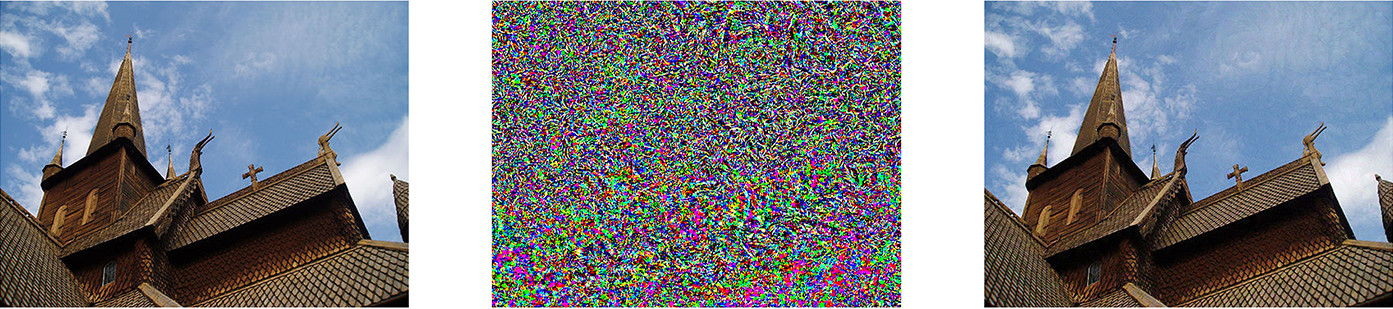
\includegraphics{{Plots/plots_robust_avg/adversarial_example_avg.jpg}}
\caption{With Perterbed Prediction Averaging, the original image on the left
was used by an adversary to create an adversarial example using $\protect%
\epsilon _{\ast }=0.02\protect\epsilon $ level noise shown in the center.
The defense averages classifications of many perturbations at $\protect%
\epsilon _{\max }=0.03\protect\epsilon $ of the example and successfuly
classifies the image despite the attack.}
\label{avg}
\end{figure*}

\section{Computational results}

\subsection{Resources}

Our computations were made using Jupyter Notebooks in Google Colaboratory
with their free GPU and TPU\ process time. All code and data interfaces are
available at the GitHub address given above, in a manner optimized for
reproducibility.

\subsection{Imagenette data}

To keep our experiments within the scope of our resources, we used a subset
of the ImageNet dataset \cite{imagenet_cvpr09} called Imagenette\footnote{%
In keeping with the wishes of the dataset curators, we ask that you
internally read \textquotedblleft Imagenette\textquotedblright\ with
\textquotedblleft a corny inauthentic French accent\textquotedblright\
unless you are in fact a native French speaker, in which case you are asked
to render it in a similarly ridiculous American accent.} \cite{imagenette}
which includes only 10 out of the original 20k classes. These classes%
\footnote{%
The classes are as follows:\ \{tench (a fish), English terrier, cassette
player, chain saw, church, French horn, garbage truck, gas pump, golf ball,
parachute\}.} are selected to be as distinct as possible, with the intention
of allowing classifiers to reach high degrees of accuracy without extensive
training for more agile experimentation.

\subsection{Neural architectures}

After testing our attack strategy with smaller convolutional networks, we
performed the work for this paper by attacking and defending two standard
models used for image classification tasks, Wide ResNet and GoogLeNet. We
took advantage of pretrained PyTorch implementations of these models and
simply restricted the output to the ten classes of interest. While the
details of these architectures are outside the scope of this review, they
can be found in \cite{zagoruyko2016wide} and \cite{szegedy2015going}.

We retrained these networks with the output node layer corrected, using 5
epochs of stochastic gradient descent with a learning rate of 0.01 and
momentum value of 0.9. This base version of Wide ResNet and GoogLeNet both
achieved 99.9\% accuracy on a test set of images. Because the results we
will show in this report are so similar for both networks, we will only show
figures related to the Wide ResNet attacks and defenses, but similar figures
for the GoogLeNet classifier and other relevant details are available in
project GitHub referenced above.

\subsection{Creating Adversarial Examples}

We applied the FGSM and DGSM\ attacks to both the Wide ResNet and GoogLeNet
classifiers with significant success. FGSM decreased accuracy in Wide ResNet
classification by more than 50\% with perturbations as small as $\epsilon
_{\ast }=0.025\epsilon $, or 2.5\% of the color range, and dropped as low as
23\% accuracy without creating perturbations obvious to the human eye.
GoogLeNet suffered worse, dropping about 73\% accuracy with an attack on the
order of $\epsilon _{\ast }=0.025\epsilon ,$ and reaching only 20\% accuracy
with $\epsilon _{\ast }=0.3\epsilon .$ These results for Wide ResNet are
shown in Figures \ref{fgsmres} and \ref{failures}. \bigskip

\begin{figure*}[h]
\centering%
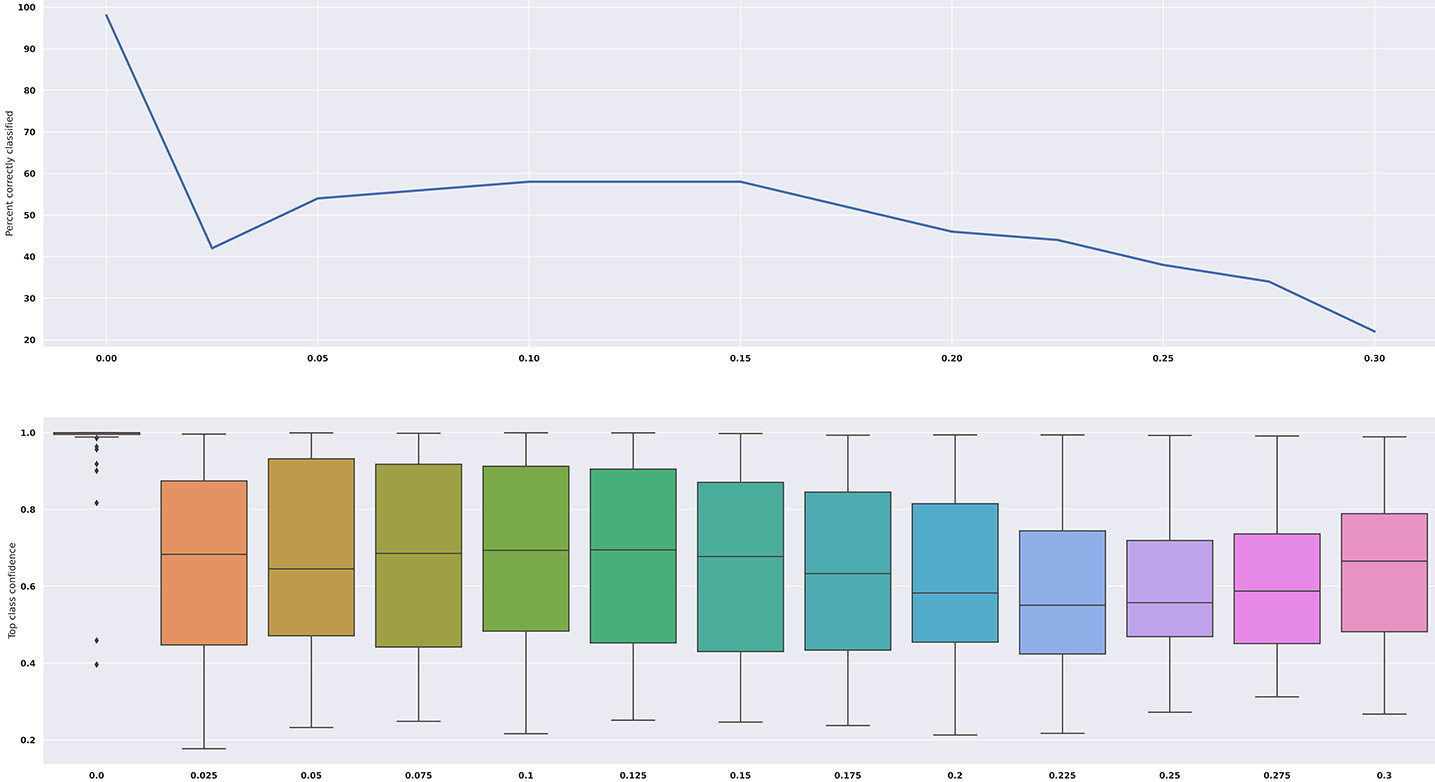
\includegraphics{{Plots/plots_base/imagenette_samples_fgsm_plots.jpg}}
\caption{Results of an FGSM attack on the Wide ResNet classifier at various
small values of $\protect\epsilon _{\ast }$.}
\label{fgsmres}
\end{figure*}

\begin{figure*}[h]
\centering%
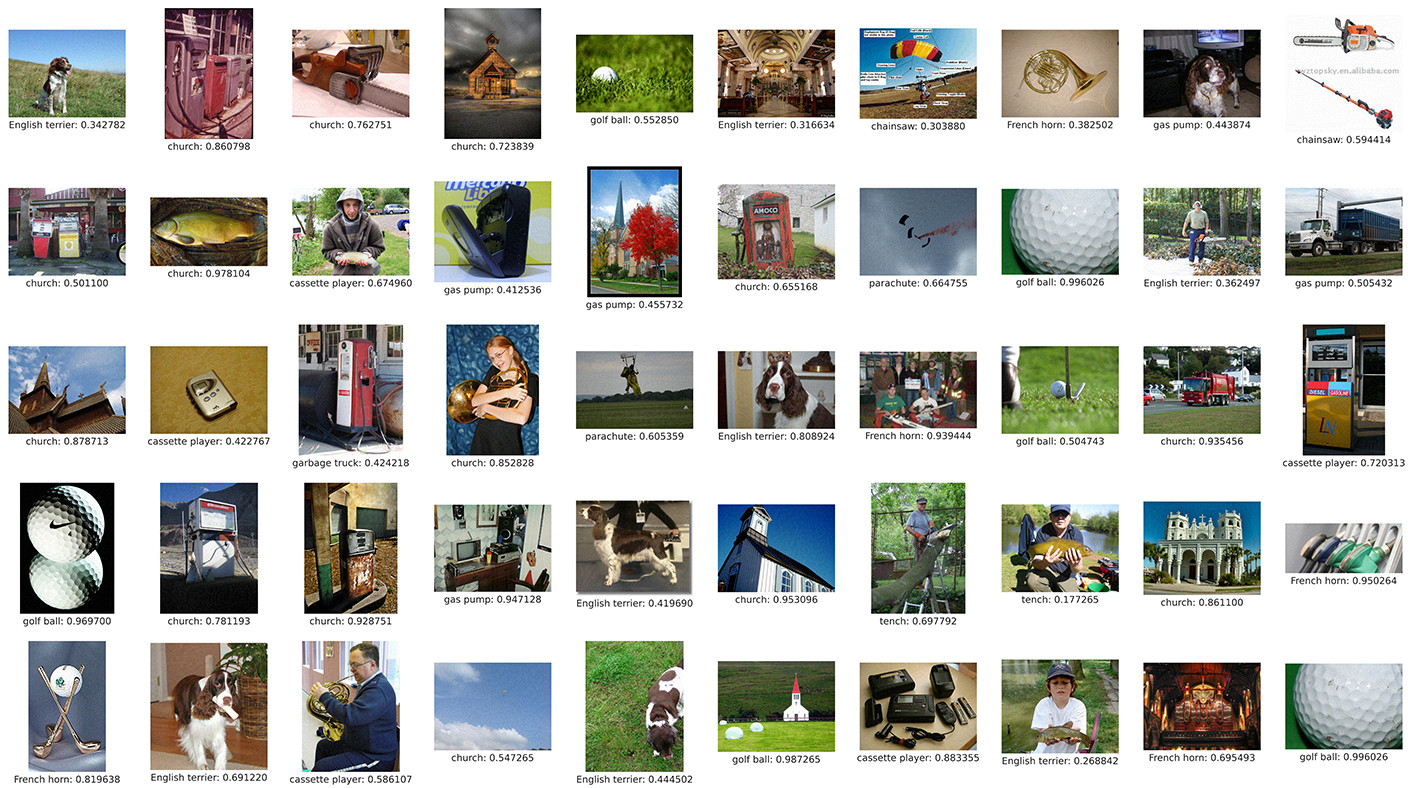
\includegraphics{{Plots/plots_base/imagenette_samples_fgsm_predictions.jpg}}
\caption{Example misclassifications made by Wide ResNet as a result of an
FGSM attack.}
\label{failures}
\end{figure*}

We then used the DGSM attack to direct the classifiers to misclassify in
favor of the English Terrier class. For both architectures we found that we
could force every image in our test set to resolve to English Terrier with
values of $\epsilon _{\ast }0.14\epsilon $ or lower, as shown for the Wide
ResNet classifier in Figure \ref{dgsm}. Interestingly, a real-world attack
of this sort would need to be cautious to weaken the attack sufficiently
that the confidence levels in classification are not so consistently high
that they give away the attack!

\begin{figure*}[h]
\centering%
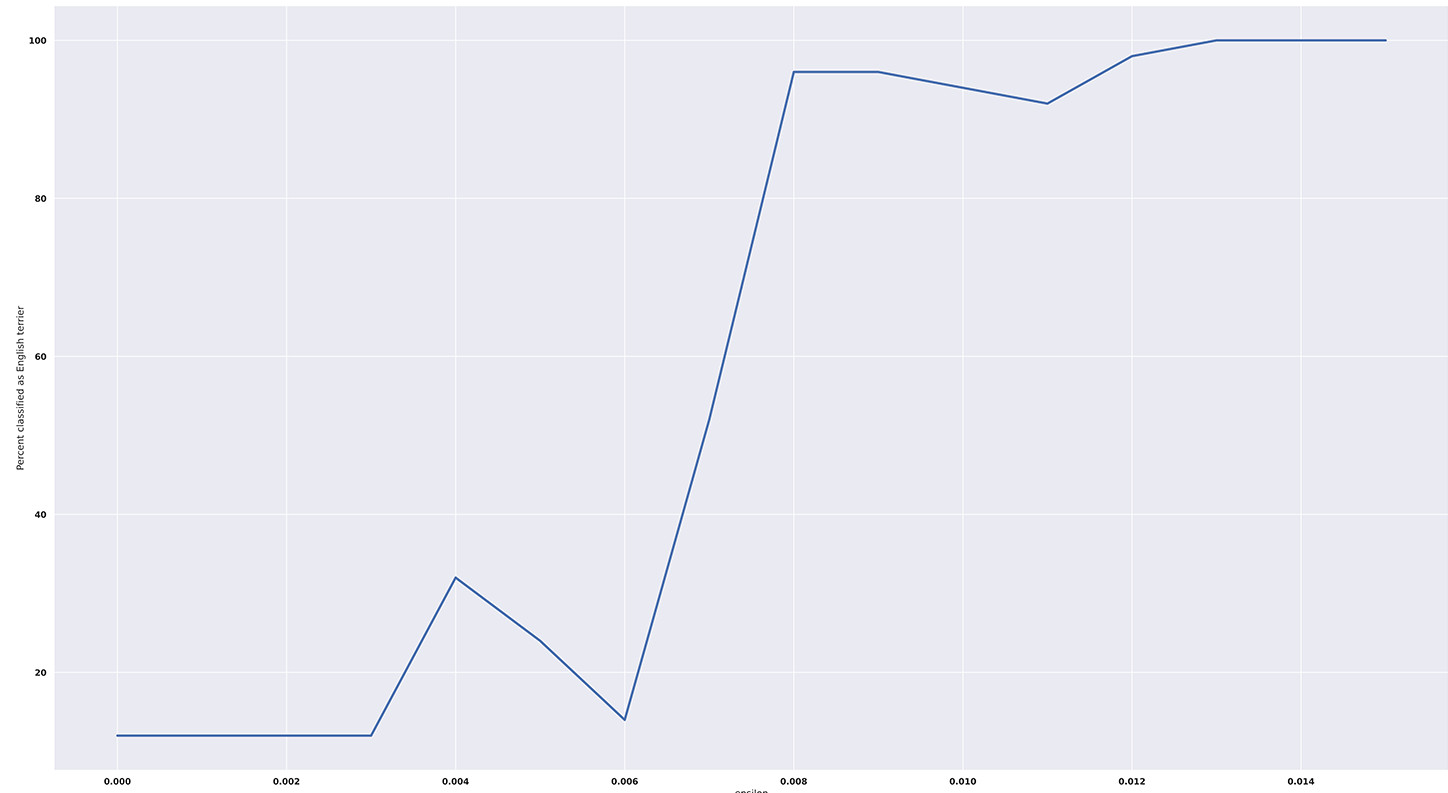
\includegraphics{{Plots/plots_base/imagenette_samples_directed_attack_plots.jpg}}
\caption{Results of a DGSM attack on the Wide ResNet classifier at various
small values of $\protect\epsilon _{\ast }$.}
\label{dgsm}
\end{figure*}

\subsection{Defenses}

For both networks we applied the Perturbed Prediction Averaging defense and
then attacked the network to see how much more robust the averaging rendered
the classifier. We found that this defense eliminated the sudden success of
very small $\epsilon _{\ast }$-sized FGSM attacks, but still allowed the
misclassification rate to grow roughly linearly with the allowed size of $%
\epsilon _{\ast }$ (see Figure \ref{ppa}).

\begin{figure*}[h]
\centering%
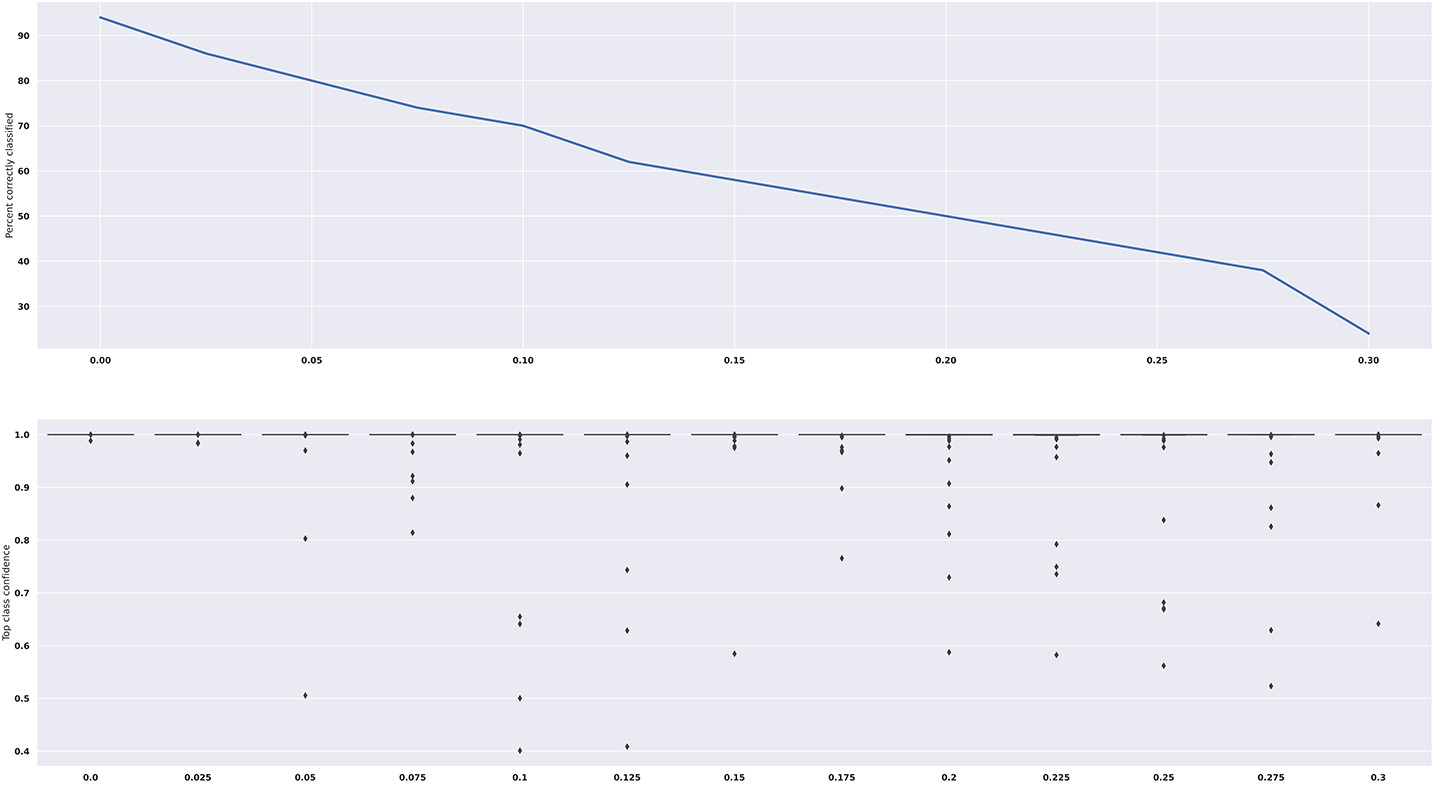
\includegraphics{{Plots/plots_robust_avg/imagenette_samples_fgsm_plots_avg.jpg}}
\caption{The classification performance loss achieved by FGSM attacks on
Wide ResNet secured with Perturbed Prediction Averaging.}
\label{ppa}
\end{figure*}
This defense proved particularly effective against the DGSM\ attack,
allowing no more than 2\% misclassification due to the attack on either
classifier.

We then repeated these tests using 10 epochs of adversarial (re)training as
our defense instead. This process reduced the overall accuracy of the Wide
ResNet classifier to 91\% and that of GoogLeNet to 70\%. This defense
improved both classifier's performance under the FGSM attack, but was more
significant for Wide ResNet (see Figure). While Wide ResNet did not dip
below 30\% accuracy until $\epsilon _{\ast }>0.1\epsilon ,$ GoogLeNet fellow
below that standard for $\epsilon _{\ast }=0.05\epsilon $. Remarkably, the
DGSM\ attack had absolutely no success on Wide ResNet when this defense was
applied, though GoogLeNet still lost as much as 4\% accuracy due to the
attack.

\begin{figure*}[h]
\centering%
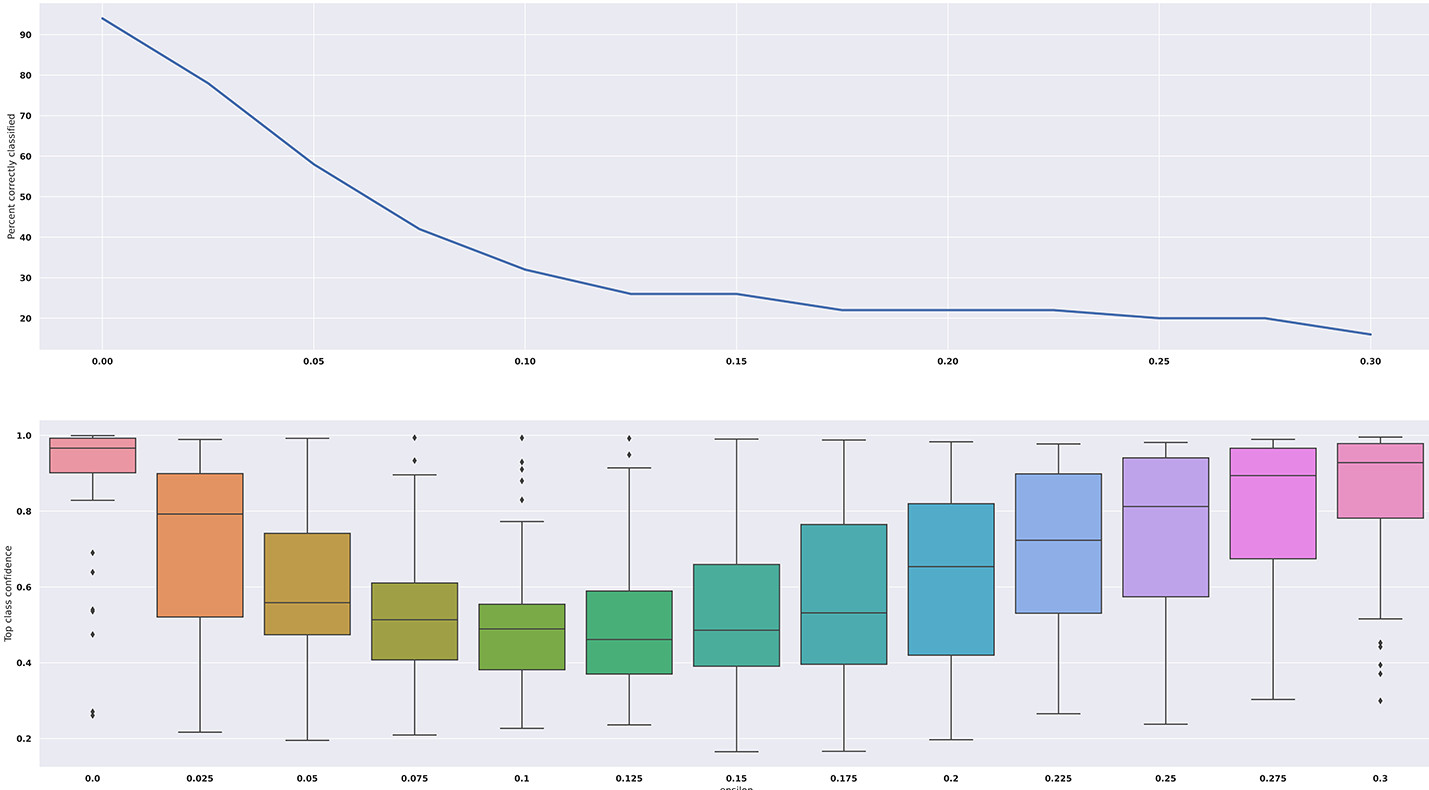
\includegraphics{{Plots/plots_robust_net/imagenette_samples_fgsm_plots_at.jpg}}
\caption{The classification performance loss achieved by FGSM attacks on
Wide ResNet secured by adversarial training.}
\label{at}
\end{figure*}

\section{Analysis}

To summarize our observations, the FGSM and DGSM\ generated adversarial
examples that successively fooled both Wide ResNet and GoogLeNet classifiers
during Imagenette classification tasks. Perturbed Prediction Averaging
performed well as an inference correction defense that would force the
adversary to use more visible perturbations to prompt similar
misclassifications with FGSM\ examples, and drastically limited DGSM\
success. Adversarial training also reduced the effect of these attacks, but
comparatively was more effective against the DGSM examples. Observing the
perturbation pattern produced by a DGSM attack (as shown in Figure \ref%
{pattern}), we noticed that it appears that the perturbation preserves
features of the image that are likely helpful for its correct
classification, at least for low enough values of $\epsilon _{\ast }$. We
speculate that this may occur because adversarial training leads to a
parameterization of the network in a region of the loss landscape that is
\textquotedblleft flatter\textquotedblright ---that is, a set of weights may
be reached by which the features extracted by deeper layers of the network
do not change very much for small changes in the input image. This idea
might be worth exploring further.

\begin{figure*}[h]
\centering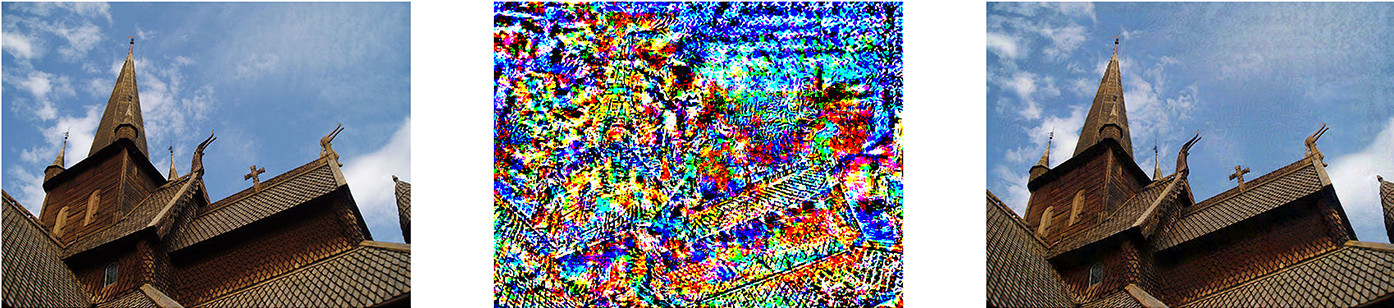
\includegraphics{{Plots/pattern_example.jpg}}
\caption{An example DGSM perturbation pattern. The $\protect\epsilon _{\ast
}=0.2\protect\epsilon $ attack captures important image features.}
\label{pattern}
\end{figure*}

There are many obvious next steps in this research that may be worth
pursuing. We did not attempt to apply both defenses at once, and it would be
interesting to see if their effects are complimentary, or if there is little
benefit. We also were very conservative in our adversarial training, and
could doubtless have improved our model accuracy by running more than 10
epochs. During our discussion about $\epsilon _{\max }$ we were
intentionally vague about our selection method. We chose $\epsilon _{\max }$
to be as small as we could assume would still allow the noise to be visible
to a human, but as we observed this parameter ought to be chosen in such a
way as to optimize the performance of the classifier with and without
adversarial attacks.

\section{Conclusions}

We have seen that adversarial examples are indeed intriguing and informative 
\cite{szegedy2014intriguing}. Image labeling is one of few tasks neural
methods seem to have essentially solved, but those fundamental linear
weaknesses highlighted by this report emphasize that the case is not closed
until defensive or corrective measures can assure classifier integrity. On
the other hand, the defenses considered are just one more addition to the
growing arsenal of network-hardening techniques readily available within the
machine learning community.

\bibliographystyle{amsplain}
\bibliography{acompat,JHU}

\end{document}
